\section{Generazione del Codice Intermedio}

In questa fase si considerano \textbf{3 aspetti} fondamentali:

\begin{itemize}
    \item \textbf{Rappresentazione intermedia}, che si divide in:
    \begin{itemize}
        \item Alberi sintattici / DAG
        \item Codice a 3 indirizzi
    \end{itemize}
    \item \textbf{Analisi sintattica} (controlli di tipo).
    \item \textbf{Generazione del codice intermedio}.
\end{itemize}

\subsection*{Flusso di compilazione (Front-end vs Back-end)}
Il seguente schema illustra il flusso dei dati attraverso i componenti del compilatore:

\begin{center}
\begin{tikzpicture}[
    node distance=1cm and 1cm,
    auto,
    block/.style={
        rectangle, 
        draw, 
        text width=2cm, 
        align=center, 
        minimum height=3em
    },
    line/.style={draw, -latex}
]

    % Nodi
    \node (start) {};
    \node [block, right=0.5cm of start] (parser) {Parser};
    \node [block, right=of parser] (checker) {Checker\\statico};
    \node [block, right=of checker] (gen_int) {Generatore\\di codice\\intermedio};
    \node [block, right=2.5cm of gen_int] (gen_cod) {Generatore\\di codice};
    \node [right=0.5cm of gen_cod] (end) {};

    % Frecce
    \path [line] (start) -- (parser);
    \path [line] (parser) -- (checker);
    \path [line] (checker) -- (gen_int);
    \path [line] (gen_int) -- node [above, font=\footnotesize] {codice} node [below, font=\footnotesize] {intermedio} (gen_cod);
    \path [line] (gen_cod) -- (end);

    % Linee Front-end / Back-end
    % Linea orizzontale sotto
    \draw [thin] ($(parser.south west) + (0,-0.8)$) -- ($(gen_cod.south east) + (0,-0.8)$);
    
    % Separatore verticale
    \draw [thick] ($(gen_int.south east) + (1.25,-0.7)$) -- ($(gen_int.south east) + (1.25,-0.9)$);
    
    % Etichette
    \node [font=\footnotesize] at ($(checker.south) + (0.5,-1.1)$) {front-end};
    \node [font=\footnotesize] at ($(gen_cod.south) + (-0.5,-1.1)$) {back-end};

\end{tikzpicture}
\end{center}

\subsection{Analisi Statica (Static Checker)}
L'analisi statica è un insieme di controlli di consistenza effettuati al momento della compilazione per garantire che il programma possa essere compilato con successo e per individuare errori prima dell'esecuzione. Si divide in:

\subsubsection{1. Controlli Sintattici}
Verificano il rispetto delle regole strutturali del linguaggio. Esempi:
\begin{itemize}
    \item Un identificatore deve essere dichiarato al più una volta nello stesso scope.
    \item Un'istruzione \texttt{break} deve trovarsi all'interno di un ciclo (\texttt{while}, \texttt{for}) o \texttt{switch}.
    \item Distinzione tra \textbf{L-value} e \textbf{R-value}:
    \begin{itemize}
        \item \textbf{L-value} (Left-value): Indica una locazione di memoria (es. a sinistra di un assegnamento: \texttt{i = 5}).
        \item \textbf{R-value} (Right-value): Indica il valore contenuto nella locazione (es. a destra di un assegnamento: \texttt{x = i + 1}).
    \end{itemize}
\end{itemize}

\subsubsection{2. Controlli di Tipo}
Garantiscono che operatori e funzioni siano applicati a un numero corretto di operandi e che il loro tipo sia adeguato.
\begin{itemize}
    \item Esempio di conversione implicita (coercion):
    \begin{itemize}
        \item \texttt{x = 4 + 5} : Nessuna conversione necessaria.
        \item \texttt{x = 4 + 5.1} : Il numero intero \texttt{4} deve essere convertito in float prima della somma.
    \end{itemize}
\end{itemize}

\subsection{Rappresentazioni Intermedie e DAG}

La rappresentazione intermedia serve da ponte tra il front-end e il back-end. Esistono diversi livelli di astrazione:

\begin{center}
\begin{tikzpicture}[node distance=0.5cm, auto, font=\small]
    % Nodi del flusso
    \node (src) {Prog. Sorgente};
    \node[right=0.8cm of src] (high) {Rapp. Alto Livello};
    \node[right=0.8cm of high] (dots) {$\dots$};
    \node[right=0.8cm of dots] (low) {Rapp. Basso Livello};
    \node[right=0.8cm of low] (tgt) {Codice Target};

    % Frecce flusso
    \draw[->] (src) -- (high);
    \draw[->] (high) -- (dots);
    \draw[->] (dots) -- (low);
    \draw[->] (low) -- (tgt);

    % Annotazioni (Albero e 3 Indirizzi)
    \node[below=0.8cm of high, text=magenta] (tree_label) {Albero Sintattico};
    \draw[->, magenta, bend right] (tree_label.north) to (high.south);

    \node[below=0.8cm of low, text=magenta] (addr_label) {Codice a 3 indirizzi};
    \node[below=0.1cm of addr_label, font=\scriptsize] {$x = y \text{ op } z$};
    \draw[->, magenta, bend right] (addr_label.north) to (low.south);
\end{tikzpicture}
\end{center}

\begin{itemize}
    \item \textbf{Albero Sintattico:} Rappresentazione gerarchica fedele alla grammatica.
    \item \textbf{DAG (Grafo Aciclico Diretto):} Simile all'albero sintattico, ma identifica le sotto-espressioni comuni. I nodi con lo stesso valore/struttura vengono riutilizzati (parte condivisa).
\end{itemize}

\subsubsection*{Esempio di DAG}
Consideriamo l'espressione: $a + a * (b - c) + (b - c) * d$.
La sotto-espressione $(b - c)$ viene calcolata una sola volta e il nodo risultante viene puntato da entrambe le parti che lo utilizzano.

\begin{center}
\begin{tikzpicture}[
    level distance=1.5cm,
    sibling distance=1.5cm,
    every node/.style={circle, inner sep=1pt},
    edge from parent/.style={draw, thick}
]

    % Definizione manuale dei nodi per creare la condivisione
    \node (root) at (0,0) {$+$};
    
    \node (plus_left) at (-2, -1.5) {$+$};
    \node (mult_right) at (2, -1.5) {$*$};
    
    \node (a_first) at (-3, -3) {$a$};
    \node (mult_left) at (-1, -3) {$*$};
    \node (d) at (3, -3) {$d$};
    
    \node (a_second) at (-2, -4.5) {$a$};
    
    % Nodo condiviso (evidenziato in rosa come negli appunti)
    \node (minus_shared) at (0, -4.5) {$-$};
    \node (b) at (-0.5, -6) {$b$};
    \node (c) at (0.5, -6) {$c$};

    % Cerchio rosa attorno alla parte condivisa
    \draw[magenta, thick] (0, -5.2) ellipse (1cm and 1.5cm);
    \node[magenta, below=1.5cm of minus_shared] {$\uparrow$ parte condivisa};

    % Collegamenti
    \draw (root) -- (plus_left);
    \draw (root) -- (mult_right);
    
    \draw (plus_left) -- (a_first);
    \draw (plus_left) -- (mult_left);
    
    \draw (mult_right) -- (minus_shared); % Condivisione destra
    \draw (mult_right) -- (d);
    
    \draw (mult_left) -- (a_second);
    \draw (mult_left) -- (minus_shared); % Condivisione sinistra
    
    \draw (minus_shared) -- (b);
    \draw (minus_shared) -- (c);

\end{tikzpicture}
\end{center}

%lezione 26 novembre
\subsection{Grafi diretti aciclici delle espressioni}

\subsubsection{Definizione guidata dalla sintassi per la costruzione di alberi sintattici e DAG}

Per costruire un grafo si utilizzano le funzioni costruttore \texttt{Leaf} e \texttt{Node}.
Per esempio, prima di costruire un nuovo nodo $Node(op, left, right)$, dobbiamo verificare se esiste un nodo con etichetta $op$ e con figli $left$ e $right$, in quest'ordine. Se tale nodo esiste la funzione $Node()$ lo restituisce, altrimenti ne crea uno nuovo.

\begin{center}
\begin{tabular}{lll}
\hline
& \textbf{Produzione} & \textbf{Regole semantiche} \\
\hline
1) & $E \to E_1 + T$ & $E.node = \textbf{new } Node('+', E_1.node, T.node)$ \\
2) & $E \to E_1 - T$ & $E.node = \textbf{new } Node('-', E_1.node, T.node)$ \\
3) & $E \to T$ & $E.node = T.node$ \\
4) & $T \to ( E )$ & $T.node = E.node$ \\
5) & $T \to \textbf{id}$ & $T.node = \textbf{new } Leaf(\textbf{id}, \textbf{id}.entry)$ \\
6) & $T \to \textbf{num}$ & $T.node = \textbf{new } Leaf(\textbf{num}, \textbf{num}.val)$ \\
\hline
\end{tabular}
\end{center}

\subsubsection{Esempio 6.2: Costruzione di un DAG complesso}

La sequenza di passi indicati di seguito costruisce il DAG mostrato nella figura successiva, a patto che le funzioni $Leaf()$ e $Node()$ ritornino un nodo già esistente, secondo quanto appena discusso, quando ciò è possibile.
Consideriamo l'espressione:
\[ a + a * (b - c) + (b - c) * d \]
\begin{figure}[H]
    \centering
    \begin{tikzpicture}[
        node distance=1.5cm,
        every node/.style={circle, draw, minimum size=0.9cm, inner sep=0pt},
        level 1/.style={sibling distance=7cm},
        level 2/.style={sibling distance=3.5cm},
        level 3/.style={sibling distance=2cm}
    ]
        % --- LIVELLO 0 (Radice) ---
        \node (p13) at (0, 0) {+};
        \node[draw=none, right=0.3cm of p13] {$p_{13}$};

        % --- LIVELLO 1 ---
        % Nodo + a sinistra
        \node (p7) at (-3.5, -1.5) {+};
        \node[draw=none, left=0.3cm of p7] {$p_7$};

        % Nodo * a destra (CORRETTO: p12)
        \node (p12) at (3.5, -1.5) {*};
        \node[draw=none, right=0.3cm of p12] {$p_{12}$};

        % --- LIVELLO 2 ---
        % Sotto p7 (+)
        \node (p1) at (-5, -3) {\textbf{a}};
        \node[draw=none, left=0.3cm of p1] {$p_1$};

        \node (p6) at (-2, -3) {*};
        \node[draw=none, right=0.3cm of p6] {$p_6$};

        % Sotto p12 (*)
        \node (p10) at (2, -3) {-};
        \node[draw=none, right=0.3cm of p10] {$p_{10}$};

        % Nodo d (CORRETTO: p11)
        \node (p11) at (5, -3) {\textbf{d}};
        \node[draw=none, right=0.3cm of p11] {$p_{11}$};

        % --- LIVELLO 3 ---
        % Sotto p6 (*)
        \node (p2) at (-3, -4.5) {\textbf{a}};
        \node[draw=none, below=0.1cm of p2] {$p_2$};

        % Nodo - di sinistra (CORRETTO: p5)
        \node (p5) at (-1, -4.5) {-};
        \node[draw=none, right=0.3cm of p5] {$p_5$};

        % Sotto p10 (-)
        % Nodo b di destra (CORRETTO: p8)
        \node (p8) at (1, -4.5) {\textbf{b}};
        \node[draw=none, below=0.1cm of p8] {$p_8$};

        \node (p9) at (3, -4.5) {\textbf{c}};
        \node[draw=none, right=0.3cm of p9] {$p_9$};

        % --- LIVELLO 4 ---
        % Sotto il nodo - di sinistra (p5)
        \node (p3) at (-2, -6) {\textbf{b}};
        \node[draw=none, below=0.1cm of p3] {$p_3$};

        \node (p4) at (0, -6) {\textbf{c}};
        \node[draw=none, below=0.1cm of p4] {$p_4$};

        % --- ARCHI ---
        \draw (p13) -- (p7);
        \draw (p13) -- (p12);

        \draw (p7) -- (p1);
        \draw (p7) -- (p6);

        \draw (p12) -- (p10);
        \draw (p12) -- (p11);

        \draw (p6) -- (p2);
        \draw (p6) -- (p5);

        \draw (p10) -- (p8);
        \draw (p10) -- (p9);

        \draw (p5) -- (p3);
        \draw (p5) -- (p4);

    \end{tikzpicture}
    \caption{L'Albero Sintattico per l'espressione $a + a * (b - c) + (b - c) * d$ senza condivisione.}
\end{figure}

Assumiamo che $entry\text{-}a$ sia un puntatore all'elemento della tabella dei simboli relativo ad \textbf{a}, e così per gli altri identificatori. Alla seconda invocazione di $Leaf(\textbf{id}, entry\text{-}a)$, alla linea 2, la funzione restituisce il puntatore al nodo precedentemente costruito, ovvero $p_2 = p_1$. Analogamente, i nodi restituiti ai passi 8 e 9 coincidono con quelli restituiti ai passi 3 e 4 (cioè $p_8 = p_3$ e $p_9 = p_4$). Di conseguenza, il nodo restituito al passo 10 deve essere lo stesso restituito al passo 5, cioè $p_{10} = p_5$.

\bigskip
\textbf{Sequenza dei puntatori:}
\begin{enumerate}
    \item $p_1 = Leaf(\textbf{id}, entry\text{-}a)$
    \item $p_2 = Leaf(\textbf{id}, entry\text{-}a) = p_1$
    \item $p_3 = Leaf(\textbf{id}, entry\text{-}b)$
    \item $p_4 = Leaf(\textbf{id}, entry\text{-}c)$
    \item $p_5 = Node('-', p_3, p_4)$
    \item $p_6 = Node('*', p_1, p_5)$
    \item $p_7 = Node('+', p_1, p_6)$
    \item $p_8 = Leaf(\textbf{id}, entry\text{-}b) = p_3$
    \item $p_9 = Leaf(\textbf{id}, entry\text{-}c) = p_4$
    \item $p_{10} = Node('-', p_3, p_4) = p_5$
    \item $p_{11} = Leaf(\textbf{id}, entry\text{-}d)$
    \item $p_{12} = Node('*', p_5, p_{11})$
    \item $p_{13} = Node('+', p_7, p_{12})$
\end{enumerate}

\bigskip
\textbf{L'Albero Sintattico (DAG) diventa:}

\begin{figure}[h!]
    \centering
    \begin{tikzpicture}[
        node distance=1.5cm,
        every node/.style={circle, draw, minimum size=0.9cm, inner sep=0pt},
        level 1/.style={sibling distance=5cm},
        level 2/.style={sibling distance=3cm}
    ]
        % Livello Radice (p13)
        \node (p13) at (0,0) {+}; 
        \node[draw=none, right=0.2cm of p13] {$p_{13}$};

        % Livello 1 (p7, p12)
        \node (p7) at (-2.5,-1.5) {+}; 
        \node[draw=none, left=0.2cm of p7] {$p_7$};
        
        \node (p12) at (2.5,-1.5) {*}; 
        \node[draw=none, right=0.2cm of p12] {$p_{12}$};

        % Livello 2 (a, p6, d)
        \node (a) at (-4,-3) {\textbf{a}}; 
        \node[draw=none, left=0.2cm of a] {$p_1, p_2$};
        
        \node (p6) at (-1,-3) {*}; 
        \node[draw=none, right=0.2cm of p6] {$p_6$};
        
        \node (d) at (4,-3) {\textbf{d}}; 
        \node[draw=none, right=0.2cm of d] {$p_{11}$};

        % Livello 3 (Nodo condiviso p5)
        \node (p5) at (1.5,-4.5) {-}; 
        \node[draw=none, right=0.2cm of p5] {$p_5, p_{10}$};

        % Livello 4 (Foglie condivise b, c)
        \node (b) at (0,-6) {\textbf{b}}; 
        \node[draw=none, left=0.2cm of b] {$p_3, p_8$};
        
        \node (c) at (3,-6) {\textbf{c}}; 
        \node[draw=none, right=0.2cm of c] {$p_4, p_9$};

        % Archi
        \draw (p13) -- (p7);
        \draw (p13) -- (p12);
        
        \draw (p7) -- (a);
        \draw (p7) -- (p6);
        
        \draw (p12) -- (p5);
        \draw (p12) -- (d);
        
        \draw (p6) -- (a); % Riuso di a
        \draw (p6) -- (p5); % Riuso di b-c
        
        \draw (p5) -- (b);
        \draw (p5) -- (c);

    \end{tikzpicture}
    \caption{DAG per l'espressione $a + a * (b - c) + (b - c) * d$.}
\end{figure}

\vspace{1 cm}
\subsection{Metodo del valore numerico per la costruzione di DAG}

Come suggerito dalla figura seguente, i nodi di un albero sintattico sono spesso memorizzati in un \textbf{Array di Record}. Ogni riga dell'array rappresenta un record e quindi un nodo. In ogni record, il primo campo è un codice operativo che indica l'etichetta del nodo.
Le foglie hanno un campo aggiuntivo contenente il valore lessicale; i nodi interni hanno due campi aggiuntivi che rappresentano i figli sinistro e destro.

In questo array ci riferiamo ai nodi mediante l'indice del record corrispondente al nodo d'interesse. Storicamente, tale indice è stato chiamato \textbf{valore numerico} o \textit{value number} del nodo o dell'espressione che esso rappresenta.
Chiamiamo \textbf{Firma (Signature)} di un nodo interno la tripla $\langle op, l, r \rangle$, in cui $op$ è l'etichetta, $l$ il valore numerico del figlio sinistro e $r$ quello del figlio destro.

\vspace{3 cm}
\textbf{Esempio:} $i = i + 10$

\begin{figure}[h!]
    \centering
    \begin{minipage}{0.45\textwidth}
        \centering
        \begin{tikzpicture}[node distance=1.5cm, auto, >=latex]
            \node[circle, draw] (eq) {=};
            \node[circle, draw, below right=of eq] (plus) {+};
            \node[draw=none, below left=of eq] (i) {i};
            \node[draw=none, below right=of plus] (ten) {10};

            \draw[->] (eq) to [bend right] (i);
            \draw[->] (eq) -- (plus);
            \draw[->] (plus) -- (i);
            \draw[->] (plus) -- (ten);
        \end{tikzpicture}
        \caption{(a) DAG}
    \end{minipage}
    \hfill
    \begin{minipage}{0.45\textwidth}
        \centering
        \begin{tabular}{|c|c|c|c|}
        \hline
        1 & \textbf{id} & \multicolumn{2}{c|}{$i$} \\ \hline
        2 & \textbf{num} & \multicolumn{2}{c|}{10} \\ \hline
        3 & + & 1 & 2 \\ \hline
        4 & = & 1 & 3 \\ \hline
        \end{tabular}
        \caption{(b) Array}
    \end{minipage}
    \caption{Nodi del DAG di $i = i + 10$ allocati in un array.}
\end{figure}

\subsubsection{Algoritmo 6.3}

\textbf{Algoritmo 6.3: Metodo del valore numerico per la costruzione dei nodi di un DAG.}

\begin{itemize}
    \item \textbf{INPUT:} L'etichetta $op$, il nodo $l$ e il nodo $r$.
    \item \textbf{OUTPUT:} Il valore numerico di un nodo nell'array con firma $\langle op, l, r \rangle$.
    \item \textbf{METODO:} Si cerchi nell'array un nodo $M$ con etichetta $op$, figlio sinistro $l$ e figlio destro $r$. Se un tale nodo esiste, si restituisca il valore numerico di $M$. Altrimenti si crei un nuovo nodo $N$ con etichetta $op$, figlio sinistro $l$ e figlio destro $r$ e si restituisca il suo valore numerico.
\end{itemize}

\subsubsection{Struttura dati per la ricerca (Tabella Hash)}

Per costruire una tabella di hash per i nodi di un DAG, abbiamo bisogno di una \textit{funzione di hash} che calcola l'indice del gruppo data una firma $\langle op, l, r \rangle$ in maniera tale da distribuire il più uniformemente possibile le firme nei vari gruppi.
Un array, indicizzato in base al valore della funzione di hash, contiene i puntatori alle teste delle varie liste.

\begin{figure}[h!]
    \centering
    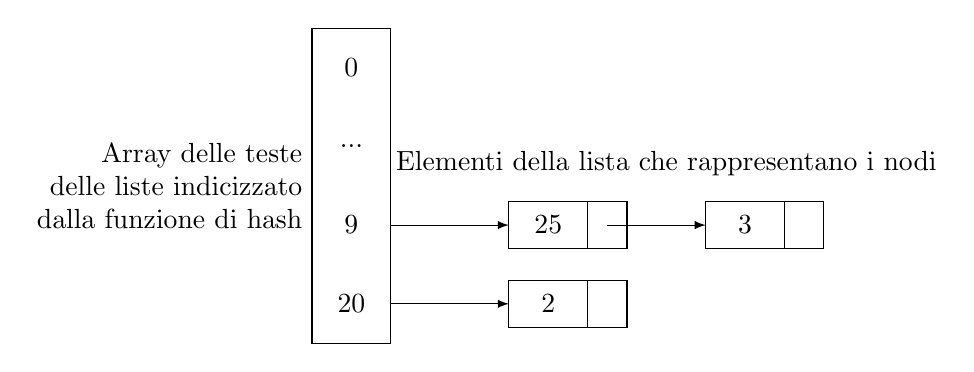
\begin{tikzpicture}
        % Array delle teste (Bucket)
        \draw (0,0) rectangle (1,4);
        \node at (0.5, 3.5) {0};
        \node at (0.5, 2.5) {...};
        \node at (0.5, 1.5) {9};
        \node at (0.5, 0.5) {20};
        \node[left, align=right] at (0, 2) {Array delle teste\\delle liste indicizzato\\dalla funzione di hash};
        
        % Bucket 9 punta alla lista
        \draw[-latex] (1, 1.5) -- (2.5, 1.5);
        \draw (2.5, 1.2) rectangle (3.5, 1.8) node[midway] {25};
        \draw (3.5, 1.2) rectangle (4.0, 1.8); 
        \draw[-latex] (3.75, 1.5) -- (5.0, 1.5);
        \draw (5.0, 1.2) rectangle (6.0, 1.8) node[midway] {3};
        \draw (6.0, 1.2) rectangle (6.5, 1.8); 
        
        % Bucket 20 punta alla lista
        \draw[-latex] (1, 0.5) -- (2.5, 0.5);
        \draw (2.5, 0.2) rectangle (3.5, 0.8) node[midway] {2};
        \draw (3.5, 0.2) rectangle (4.0, 0.8);
        
        \node[above] at (4.5, 2) {Elementi della lista che rappresentano i nodi};
    \end{tikzpicture}
    \caption{Struttura dati per la ricerca degli elementi in un gruppo.}
\end{figure}

La ricerca del VN di una firma $\langle op, l, r \rangle$ procede cercando il nodo richiesto all'interno della lista $h(\langle op, l, r \rangle)$.
\begin{itemize}
    \item Si scorre la lista alla ricerca di un elemento la cui firma sia $\langle op, l, r \rangle$.
    \item \textbf{SE} si trova un tale elemento, se ne restituisce il valore numerico.
    \item \textbf{ALTRIMENTI}, si aggiunge alla lista un elemento con firma $\langle op, l, r \rangle$ e se ne restituisce il VN.
\end{itemize}

\subsection{Codice a 3 Indirizzi}

Esempio:
\begin{verbatim}
x = y op z
x + y * z
    t1 = y * z
    t2 = x + t1
\end{verbatim}

Il seguente codice a tre indirizzi è derivato direttamente dalla struttura del DAG mostrato sopra. Notare come le variabili temporanee riutilizzino i risultati comuni (come $t_1$).

\begin{verbatim}
t1 = b - c
t2 = a * t1
t3 = a + t2
t4 = t1 * d
t5 = t3 + t4
\end{verbatim}

Consideriamo ora le più comuni istruzioni a tre indirizzi che utilizzeremo nel resto di questa trattazione.
Un indirizzo può assumere una delle seguenti forme:
\begin{enumerate}
    \item \textbf{Un nome.} Per comodità, nel codice a tre indirizzi utilizzeremo direttamente i nomi degli identificatori così come appaiono nel codice sorgente.
    \item \textbf{Una costante.} In pratica un compilatore deve trattare molti tipi diversi di costanti e variabili.
    \item \textbf{Un nome temporaneo} generato dal compilatore, ogni volta che una variabile temporanea sia necessaria.
\end{enumerate}

\subsubsection{Le istruzioni più comuni}

\begin{enumerate}
    \item \textbf{Istruzioni di assegnamento del tipo $x = y \ op \ z$}, in cui $op$ è un operatore binario aritmetico o logico e $x$, $y$ e $z$ sono indirizzi.
    
    \item \textbf{Istruzioni di assegnamento del tipo $x = op \ z$}, in cui $op$ indica un'operazione unaria. (Es. meno unario, la negazione logica.)
    
    \item \textbf{Istruzioni di copia del tipo $x = y$}, secondo cui a $x$ viene assegnato il valore di $y$.
    
    \item \textbf{Istruzioni di salto incondizionato del tipo \texttt{goto L}}, secondo cui la successiva istruzione a essere eseguita sarà quella con etichetta simbolica $L$.
    
    \item \textbf{Istruzioni di salto condizionato del tipo \texttt{if x goto L} oppure \texttt{ifFalse x goto L}}. Queste istruzioni fanno sì che l'istruzione successiva a essere eseguita sia quella indicata dall'etichetta $L$ se la condizione $x$ è rispettivamente vera oppure falsa. In entrambi i casi, qualora la condizione non sia soddisfatta sarà l'istruzione immediatamente successiva a essere eseguita, seguendo pertanto il normale flusso di esecuzione.
    
    \item \textbf{Istruzioni di salto condizionato del tipo \texttt{if x relop y goto L}}. Tali istruzioni applicano l'operatore relazionale $relop$ ($<, \le, ==, \dots$) agli operandi $x$ e $y$; se tali operandi soddisfano la relazione indicata esse fanno sì che la successiva istruzione a essere eseguita sia quella con etichetta $L$. In caso contrario, sarà l'istruzione immediatamente successiva a essere eseguita, seguendo pertanto il normale flusso di esecuzione.
    
    \item \textbf{Chiamata di procedura e ritorno da procedura.} Le chiamate di procedura sono implementate mediante una istruzione \texttt{param x} per ogni parametro, una istruzione \texttt{call p, n} oppure \texttt{y = call p, n} per la chiamata vera e propria della procedura o della funzione e, infine, una istruzione \texttt{return y} -- in cui l'indirizzo $y$ è opzionale -- che indica il valore restituito al chiamante.
    \\
    Generata in corrispondenza della chiamata di procedura $p(x_1, x_2, \dots, x_n)$. Il valore intero $n$, che indica il numero dei parametri in una chiamata del tipo \texttt{call p, n}, non è ridondante, poiché le chiamate possono essere annidate. In altre parole può accadere che alcune delle prime istruzioni \texttt{param} siano parte di una chiamata che avviene dopo che $p$ ha restituito il suo valore, che diviene pertanto un ulteriore parametro per la seconda chiamata. 
    
    \item \textbf{Istruzioni di copia indicizzata del tipo $x = y[i]$ oppure $x[i] = y$}. La prima istruzione assegna a $x$ il valore che si trova $i$ posizioni dopo la locazione di memoria indicata da $y$. Analogamente, la seconda istruzione assegna il valore $y$ alla locazione di memoria che si trova $i$ posizioni dopo quella relativa a $x$.
    
    \item \textbf{Assegnamenti di puntatori e indirizzi del tipo $x = \&y$, $x = *y$ oppure $*x = y$}. 
    L'istruzione $x = \&y$ assegna a $x$, precisamente all'r-value di $x$, l'indirizzo di $y$, cioè il suo l-value. Presumibilmente $y$ è un nome, eventualmente temporaneo, che denota una espressione avente un l-value definito, come \texttt{A[i][j]}, mentre $x$ è il nome di un puntatore oppure una variabile temporanea. 
    Nell'istruzione $x = *y$, presumibilmente $y$ è un puntatore o una variabile temporanea il cui r-value indica una locazione di memoria; in tal caso $x$ (il suo r-value) assume il valore di tale locazione. 
    Infine, l'istruzione $*x = y$ assegna il valore di $y$ all'r-value dell'oggetto puntato da $x$.
\end{enumerate}


%lezione 27 novembre
\textbf{Esempio 6.5.} Si consideri lo statement:
$$ do \ i = i + 1; \ while \ (a[i] < v); $$

Due possibili traduzioni sono mostrate nella figura seguente. La soluzione (a) utilizza un'etichetta simbolica $L$ associata alla prima istruzione. La traduzione (b) utilizza i numeri delle posizioni delle istruzioni, iniziando arbitrariamente a 100. In entrambi i casi l'ultima istruzione è un salto condizionato alla prima istruzione.

\subsubsection*{Nota}
La moltiplicazione $i * 8$ sottintende che la dimensione di ogni elemento dell'array abbia dimensioni pari a 8 unità.


\begin{table}[H]
\centering
\begin{tabular}{l|l}
\textbf{(a) Etichette simboliche} & \textbf{(b) Indici di posizione} \\
\hline
\begin{minipage}{6cm}
\vspace{0.2cm}
L: \quad $t_1 = i + 1$ \\
\hspace*{0.6cm} $i = t_1$ \\
\hspace*{0.6cm} $t_2 = i * 8$ \\
\hspace*{0.6cm} $t_3 = a[t_2]$ \\
\hspace*{0.6cm} if $t_3 < v \ goto \ L$
\vspace{0.2cm}
\end{minipage}
&
\begin{minipage}{6cm}
\vspace{0.2cm}
100: \ $t_1 = i + 1$ \\
101: \ $i = t_1$ \\
102: \ $t_2 = i * 8$ \\
103: \ $t_3 = a[t_2]$ \\
104: \ if $t_3 < v \ goto \ 100$
\vspace{0.2cm}
\end{minipage}
\end{tabular}
\caption{Due metodi per l'assegnamento delle etichette a una sequenza di istruzioni a tre indirizzi }
\end{table}

La scelta di quali operatori utilizzare nella rappresentazione intermedia è cruciale. L'insieme deve essere sufficientemente ricco da consentire l'implementazione di tutte le operazioni del linguaggio sorgente.

\subsection{Rappresentazione del Codice Intermedio}

Le istruzioni a tre indirizzi possono essere implementate come record. Tre comuni rappresentazioni sono le \textbf{quadruple}, le \textbf{triple} e le \textbf{triple indirette}.

\subsubsection{1. Quadruple}
Una quadrupla (o \textit{quad}) ha quattro campi: $op$, $arg_1$, $arg_2$ e $result$.
Il campo $op$ contiene un codice interno che indica l'operatore.
Esempio: $x = y + z$ è rappresentato con $+$, $y$, $z$, $x$.

\textbf{Eccezioni:}
\begin{itemize}
    \item Istruzioni con operatori unari (es. $x = \text{minus } y$) o copie ($x=y$) non usano $arg_2$. Per le copie, $op$ è l'assegnamento.
    \item Istruzioni come $param \ x$ non usano né $arg_2$ né $result$.
    \item I salti condizionati e incondizionati salvano l'etichetta in $result$.
\end{itemize}

\textbf{Esempio:} $a = b * -c + b * -c$

\begin{table}[H]
\centering
\begin{tabular}{|c|c|c|c|c|}
\hline
 & \textbf{op} & \textbf{arg$_1$} & \textbf{arg$_2$} & \textbf{result} \\
\hline
0 & minus & c & & $t_1$ \\
1 & * & b & $t_1$ & $t_2$ \\
2 & minus & c & & $t_3$ \\
3 & * & b & $t_3$ & $t_4$ \\
4 & + & $t_2$ & $t_4$ & $t_5$ \\
5 & = & $t_5$ & & a \\
\hline
\end{tabular}
\caption{Rappresentazione tramite Quadruple. Si nota come il "minus" unario sia distinto dalla sottrazione.}
\end{table}

\subsubsection{2. Triple}
Una tripla è un record con soli tre campi: $op$, $arg_1$ e $arg_2$.
Il campo $result$ è utilizzato principalmente da variabili temporanee, quindi viene eliminato. Ci si riferisce al risultato di un'operazione mediante la sua \textbf{posizione} nella sequenza di codice (es. $(0)$, $(1)$).

Le triple sono equivalenti alla struttura di un \textbf{DAG} (Albero Sintattico).

\begin{figure}[H]
\centering
\begin{minipage}{0.45\textwidth}
    \centering
    \begin{tikzpicture}[
        level distance=1.2cm, % Aumentato leggermente per leggibilità verticale
        level 1/.style={sibling distance=4cm}, % Molto spazio tra 'a' e il blocco '+'
        level 2/.style={sibling distance=2.5cm}, % Spazio tra i due '*' per evitare collisioni sotto
        level 3/.style={sibling distance=1.2cm}  % Spazio normale tra 'b' e 'minus'
    ]
    \node {=}
        child {node {a}}
        child {node {+}
            child {node {*}
                child {node {b}}
                child {node {minus} child {node {c}}}
            }
            child {node {*}
                child {node {b}}
                child {node {minus} child {node {c}}}
            }
        };
    \end{tikzpicture}
    \caption{Albero Sintattico}
    \end{minipage}
\hfill
\begin{minipage}{0.45\textwidth}
\centering
\begin{tabular}{|c|c|c|c|}
\hline
 & \textbf{op} & \textbf{arg$_1$} & \textbf{arg$_2$} \\
\hline
0 & minus & c & \\
1 & * & b & (0) \\
2 & minus & c & \\
3 & * & b & (2) \\
4 & + & (1) & (3) \\
5 & = & a & (4) \\
\hline
\end{tabular}
\caption{Tabella delle Triple }
\end{minipage}
\end{figure}

L'istruzione di copia $a=t_5$, nella notazione a triple è codificato ponendo $a$ in $arg_1$ e il valore numerico $(4)$ in $arg_2$.

\subsubsection{3. Triple Indirette}
Uno svantaggio delle triple, rispetto alle quadruple, emerge nei compilatori ottimizzanti. Se spostiamo un'istruzione, dobbiamo modificare tutti i riferimenti al suo indice.
Le \textbf{triple indirette} risolvono il problema usando una lista di puntatori alle triple (array \textit{instruction}).
L'ottimizzatore può spostare l'istruzione modificando l'ordine in \textit{instruction}, senza toccare le triple stesse.

\textbf{Esempio:} Istruzione $z = (x+y) * (10+w)$;

\vspace{0.5cm}

% Parte superiore: Confronto tra ordine originale e riordinato
\begin{center}
\begin{tabular}{p{3cm} c c c c}
\textbf{3 Istruzioni} & \textbf{Triple (Originali)} & & \textbf{Esecuzione Riordinata} & \\
$t_1: x+y$     & 0: + x y     & & + 10 w & \\
$t_2: 10+w$    & 1: + 10 w    & $\xrightarrow{\text{CAMBIO ORDINE}}$ & + x y & \\
$t_3: t_1 * t_2$ & 2: * (0) (1) & & * (1) (0) & \\
$z: t_3$       & 3: = z (2)   & & = z (2) & \\
\end{tabular}
\end{center}

\vspace{0.8cm}

% Parte inferiore: Array Instruction
\noindent \textbf{Array Instruction:}

\begin{center}
\begin{minipage}{0.2\textwidth}
    \centering
    (0) \\
    (1) \\
    (2) \\
    (3)
\end{minipage}
\begin{minipage}{0.1\textwidth}
    \centering
    $\longrightarrow$
\end{minipage}
\begin{minipage}{0.2\textwidth}
    \centering
    (1) \\
    (0) \\
    (2) \\
    (3)
\end{minipage}
\begin{minipage}{0.35\textwidth}
    \small $\rightarrow$ I puntatori nelle triple non cambiano, cambia solo l'ordine nell'array.
\end{minipage}
\end{center}

\subsection{Tipi e Dichiarazioni}

L'uso dei tipi ha diversi obiettivi, raggruppabili in due classi:

\begin{itemize}
    \item \textbf{Controllo di tipo (Type Checking):} Il controllo di tipo utilizza regole logiche per analizzare staticamente il comportamento di un programma al momento della sua esecuzione. Specificamente, garantisce che i tipi degli operandi siano quelli adatti al relativo operatore. 
    
    \item \textbf{Traduzione:} In base al tipo di un determinato nome, il compilatore può determinare lo spazio di memoria necessario a run-time. Inoltre, le informazioni di tipo sono necessarie per calcolare l'indirizzo relativo a un elemento di un array, per conversioni di tipo, ecc.
\end{itemize}

\vspace{0.3cm}

\noindent \textbf{Organizzazione della memoria:} La memoria per i nomi dichiarati all'interno di una procedura o di una classe è allocata durante l'esecuzione. Tuttavia, a compile-time, definiamo l'organizzazione ricorrendo a \textit{indirizzi relativi} (offset). L'indirizzo relativo è uno spiazzamento rispetto all'inizio della zona dati.

\subsubsection{Espressioni di Tipo}

I tipi hanno una struttura ben precisa che rappresenteremo mediante le \textit{espressioni di tipo}, di cui useremo la seguente definizione.
\begin{itemize}
    \item Un \textbf{tipo di base} è un'espressione di tipo (es. \textit{boolean, char, integer, float, void}).
    \item Un \textbf{nome di tipo} è un'espressione di tipo.
    \item Un'espressione di tipo può essere costruita applicando il costruttore di tipo \textbf{array} a un intero e a un'espressione di tipo.
    \item Un \textbf{record} è una struttura dati composta da campi aventi un nome. Si applica il costruttore \textit{record} ai nomi dei campi e ai loro tipi.
    \item Un'espressione può essere ottenuta applicando il costruttore di tipo $\rightarrow$ relativo ai tipi delle funzioni. Scriviamo $s \rightarrow t$ per indicare una funzione dal tipo $s$ (argomenti) al tipo $t$ (valore restituito).
    \item Se $s$ e $t$ sono espressioni di tipo, anche il loro \textbf{prodotto cartesiano} $s \times t$ è un'espressione di tipo.
    \begin{quote}
        \textit{\small $\rightarrow$ Nota : Serve per formare coppie e può essere usato più volte (es. liste o tuple).}
    \end{quote}
    \item Le espressioni di tipo possono contenere variabili i cui valori sono altre espressioni di tipo.
\end{itemize}

\vspace{0.5cm}

\subsubsection{Tipi Ricorsivi}
È un tipo di dato che fa riferimento a sé stesso nelle proprie definizioni.

$$ LIST = Nil \ | \ integer \times LIST $$

\noindent \textbf{Rappresentazione grafica (Grafo dei tipi):}

\begin{center}
\begin{tikzpicture}[>=Stealth, node distance=1.5cm, auto]
    % Stile dei nodi come nel disegno (ellissi)
    \node[draw, ellipse, thick, minimum width=1.5cm] (list) {LIST};
    \node[draw, ellipse, thick, minimum width=1cm, below left=1.5cm of list] (nil) {Nil};
    
    % Nodo prodotto cartesiano (cerchio con X)
    \node[draw, circle, thick, inner sep=2pt, below right=1.5cm of list] (cross) {$\times$};
    
    % Nodo integer
    \node[draw, ellipse, thick, minimum width=1.5cm, below=1.5cm of cross] (int) {integer};

    % Archi
    \draw[->, thick] (list) -- (nil);
    \draw[->, thick] (list) -- (cross);
    \draw[->, thick] (cross) -- (int);
    
    % Arco curvo di ritorno (ricorsione)
    \draw[->, thick] (cross) to[out=45, in=0] (list);
\end{tikzpicture}
\end{center}

\subsubsection{Equivalenza di Tipo}
Due espressioni di tipo sono strutturalmente equivalenti se e solo se:
\begin{enumerate}
    \item Sono lo stesso tipo di base.
    \item Sono ottenute applicando lo stesso costruttore di tipo a espressioni strutturalmente equivalenti a due a due.
    \item Una è un nome di tipo che indica l'altra.
\end{enumerate}
Se i nomi di tipo fossero interpretati come se rappresentassero loro stessi, le prime due condizioni della definizione appena citata portano al concetto di equivalenza per nome.


\subsubsection{Grammatica per le Dichiarazioni}

Studiamo i tipi utilizzando una grammatica semplificata, che dichiara un solo nome alla volta:

\begin{align*}
D &\to T \ id ; \ D \ | \ \epsilon \\
T &\to B \ C \ | \ record \ \{ D \} \\
B &\to int \ | \ float \\
C &\to [num] \ C \ | \ \epsilon
\end{align*}
\begin{itemize}
    \item Il non-terminale $D$ genera dichiarazioni.
    \item Il non-terminale $T$ genera tipi base, array e record.
    \item Il non-terminale $B$ genera uno dei due tipi di base (int e float).
    \item Il non-terminale $C$ (componente) genera stringhe di zero o più interi.
    \item Un tipo array consiste di un tipo di base specificato da B seguito dalle componenti descritte da C.
    \item Un tipo record (la seconda produzione relativa a T) è una sequenza di dichiarazioni relative ai diversi campi del record racchiuse tra parentesi graffe 
\end{itemize}    
    

\subsubsection{Organizzazione della Memoria per i nomi locali}
Dal nome di un tipo possiamo determinare la quantità di memoria che sarà necessaria a run-time per memorizzare valori associati a quel nome. A compile-time, possiamo utilizzare le informazioni relative al tipo per assegnare a ogni nome un indirizzo relativo.

Il tipo e l'indirizzo relativo di un certo nome sono memorizzati nell'elemento della tabella dei simboli relativo a quel nome. I dati di dimensione variabile (per esempio, le stringhe) o quelli la cui dimensione non può essere determinata se non al momento dell'esecuzione (per esempio, gli array dinamici) sono gestiti riservando solamente una quantità di memoria nota a priori e destinata a contenere un puntatore ai dati veri e propri.

Supponiamo che la memoria sia organizzata in blocchi contigui di più byte, nell'ipotesi che il byte sia la più piccola unità di memoria indirizzabile.

La \textit{larghezza} di un tipo indica il numero di unità di memorizzazione (\textbf{BYTE}) necessarie per un oggetto di quel tipo. I tipi di base (interi, caratteri, valori in virgola mobile) richiedono un numero intero di byte.

Per semplificare l'accesso, l'organizzazione della memoria relativa a tipi aggregati quali array e classi prevede un'allocazione contigua in un unico blocco.

\vspace{0.5cm}

\color{blue} % Colore blu per simulare la penna, opzionale (richiede package xcolor)
\textbf{ALLINEAMENTO:} \color{black}Porta ad un surplus di byte (\textit{PADDING}). \\
$\hookrightarrow$ ES: i 2 byte sprecati per allineare.
\color{black}

\vspace{0.5cm}


\subsubsection{SDT PER CALCOLARE IL TIPO (TYPE) E LA LARGHEZZA (WIDTH) PER I TIPI BASE E GLI ARRAY}

Lo SDT utilizza gli attributi sintetizzati $type$ e $width$ per ogni non-terminale e due variabili $t$ e $w$ per passare le informazioni di tipo e larghezza da un nodo $B$ nell'albero di parsing al nodo relativo alla produzione $C \to \epsilon$. In una definizione guidata dalla sintassi $t$ e $w$ sarebbero attributi ereditati di $C$.

\begin{align*}
T &\to B \quad \{ t = B.type; \ w = B.width; \} \\
  &\quad \ \ C \quad \{ T.type = C.type; \ T.width = C.width; \} \\[1em]
B &\to \mathbf{int} \quad \{ B.type = integer; \ B.width = 4; \} \\
B &\to \mathbf{float} \quad \{ B.type = float; \ B.width = 8; \} \\[1em]
C &\to \epsilon \quad \{ C.type = t; \ C.width = w; \} \\
C &\to [\mathbf{num}] \ C_1 \quad \{ C.type = array(\mathbf{num}.value, C_1.type); \\
  &\quad \quad \quad \quad \quad \quad \quad C.width = \mathbf{num}.value \times C_1.width; \}
\end{align*}

\vspace{0.3cm}
\noindent \textbf{Spiegazione:}
\begin{itemize}
    \item Il corpo della produzione per $T$ assegna $B.type$ a $t$ e $B.width$ a $w$.
    \item Le produzioni per $C$ determinano se $T$ genera un tipo base o un array.
    \item Se $C \to \epsilon$, allora $t$ e $w$ diventano gli attributi di $C$.
    \item Se $C \to [\mathbf{num}] C_1$, si costruisce l'array e si moltiplica la larghezza: $width = \text{num.value} \times C_1.width$.
\end{itemize}

\vspace{0.5cm}
\noindent \textbf{Esempio: \texttt{int[2][3]}}
\\ Le linee tratteggiate mostrano l'albero di parsing. Le linee continue e le frecce mostrano la propagazione degli attributi: $t, w$ scendono (ereditati) verso destra, mentre $type, width$ risalgono (sintetizzati) verso sinistra.
\begin{center}
    \begin{tikzpicture}[scale=1, transform shape]
        % --- COORDINATE CALCOLATE PER PARALLELISMO PERFETTO ---
        \coordinate (T) at (0, 0);
        \coordinate (B) at (-4, -2);
        \coordinate (C1) at (2, -2);
        \coordinate (C2) at (5, -5);
        \coordinate (C3) at (8, -8);
        \coordinate (Eps) at (8, -9.2);
    
        % --- RAMI DELL'ALBERO (Tratteggiati) ---
        \draw[dotted, thick] (T) -- (B);
        \draw[dotted, thick] (B) -- +(-0.5, -0.8) node[below] {\textbf{int}};
        
        \draw[dotted, thick] (T) -- (C1);
        \draw[dotted, thick] (C1) -- +(-1, -1) node[below] {$[2]$};
        \draw[dotted, thick] (C1) -- (C2);
        \draw[dotted, thick] (C2) -- +(-1, -1) node[below] {$[3]$};
        \draw[dotted, thick] (C2) -- (C3);
        \draw[dotted, thick] (C3) -- (Eps) node[below] {$\boldsymbol{\epsilon}$};
    
        % --- NODI ---
        \node[fill=white, inner sep=1pt] at (T) {$T$};
        \node[fill=white, inner sep=1pt] at (B) {$B$}; 
        \node[fill=white, inner sep=1pt] at (C1) {$C$}; 
        \node[fill=white, inner sep=1pt] at (C2) {$C$}; 
        \node[fill=white, inner sep=1pt] at (C3) {$C$};
    
        % --- TESTI DEGLI ATTRIBUTI ---
        
        % 1. Testo B
        \node[align=left, font=\scriptsize] (TxtB) at (-5, -1.5) 
            {$type=integer$ \\ $width=4$};
    
        % 2. Testo T
        \node[align=left, font=\scriptsize] (TxtT) at (2.5, 0.5) 
            {$type=array(2, array(3, integer))$ \\ $width=24$};
    
        % 3. Testo C1
        \node[align=left, font=\scriptsize] (TxtC1) at (4.5, -1.5) 
            {$type=array(2, array(3, integer))$ \\ $width=24$};
    
        % 4. Testo C2
        \node[align=left, font=\scriptsize] (TxtC2) at (7.5, -4.5) 
            {$type=array(3, integer)$ \\ $width=12$};
    
        % 5. Testo C3
        \node[align=left, font=\scriptsize] (TxtC3) at (10.5, -7.5) 
            {$type=integer$ \\ $width=4$};
    
        % --- FRECCE ---
    
        % 1. FRECCIA EREDITATA (Discendente)
        % CORREZIONE: aggiunto 'align=center' qui sotto per risolvere l'errore
        \draw[->, >=latex, thick] (-3, -1.5) to[out=20, in=150] 
            node[midway, above, font=\scriptsize, align=center] {$t=integer$ \\ $w=4$} 
            (1.5, -1.8);
    
        % 2. FRECCE SINTETIZZATE (Ascendenti - Parallele)
        
        % Da C3 a C2
        \draw[->, >=latex, thick] (TxtC3.north west) -- (TxtC2.south east);
        
        % Da C2 a C1
        \draw[->, >=latex, thick] (TxtC2.north west) -- (TxtC1.south east);
        
        % Da C1 a T
        \draw[->, >=latex, thick] (TxtC1.north west) -- (TxtT.south east);
    
    \end{tikzpicture}
    \end{center}

\subsection{SEQUENZE DI DICHIARAZIONI}

Prima che la prima delle dichiarazioni sia analizzata, il valore della variabile \textit{offset} viene inizializzato a 0. Ogni volta che viene individuato un nuovo nome, esso viene inserito nella tabella dei simboli con l'offset corrente, incrementato poi della larghezza del tipo.

\begin{align*}
P &\to \quad \{ offset = 0; \} \\
  &\quad \ \ D \\[1em]
D &\to T \ \mathbf{id} ; \quad \{ top.put(\mathbf{id}.lexeme, T.type, offset); \\
  &\quad \quad \quad \quad \quad \quad offset = offset + T.width; \} \\
  &\quad \ \ D_1 \\[1em]
D &\to \epsilon
\end{align*}

\vspace{0.5cm}
\noindent \textbf{Esempio :}

\begin{center}
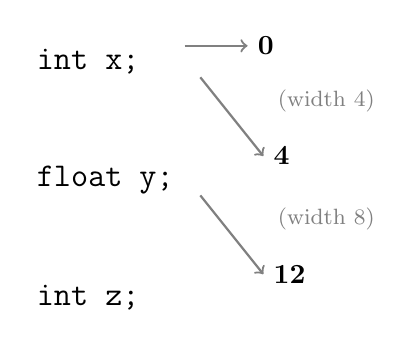
\begin{tikzpicture}[x=1cm, y=1cm]
    % Codice
    \node[anchor=west, font=\large] at (0, 3) {\texttt{int x;}};
    \node[anchor=west, font=\large] at (0, 1.5) {\texttt{float y;}};
    \node[anchor=west, font=\large] at (0, 0) {\texttt{int z;}};

    % Frecce e valori offset
    \draw[->, gray, thick] (2, 3.2) -- (2.8, 3.2) node[right, black] {\textbf{0}};
    
    \draw[->, gray, thick] (2.2, 2.8) -- (3, 1.8) node[right, black] {\textbf{4}}; 
    \node[text=gray, font=\footnotesize] at (3.8, 2.5) {(width 4)};

    \draw[->, gray, thick] (2.2, 1.3) -- (3, 0.3) node[right, black] {\textbf{12}};
    \node[text=gray, font=\footnotesize] at (3.8, 1) {(width 8)};

\end{tikzpicture}
\end{center}

\subsection{CAMPI NEI RECORD E NELLE CLASSI}

La produzione che ci interessa è:
$$ T \to \mathbf{record} \ '\{' \ D \ '\}' $$

Un approccio simile a quello delle dichiarazioni può essere esteso ai tipi e agli indirizzi relativi ai campi, a patto che siano soddisfatte due condizioni:
\begin{itemize}
    \item I nomi dei campi di un record devono essere tutti distinti (cioè ogni nome può apparire una sola volta nelle dichiarazioni generate da $D$).
    \item L'indirizzo relativo è dato rispetto all'indirizzo di base dello specifico record.
\end{itemize}

Per comodità ogni tipo record utilizzerà una tabella dei simboli locale per memorizzare le informazioni relative a tipo e indirizzo relativo dei suoi campi. Un tipo record ha la
forma record (t) in cui record() è il costruttore di tipo e t è un oggetto che rappresenta
la tabella dei simboli contenente tutte le informazioni relative ai campi del record.

\vspace{0.3cm}
\noindent \textbf{Esempio :}
L'uso di un nome $x$ per indicare un campo di un record non entra in conflitto con altri usi dello stesso nome al di fuori del record.

\begin{verbatim}
    float x;
    record { float x; float y; } p;
    record { int tag; float x; float y; } q;
\end{verbatim}